\documentclass[tikz,border=10pt]{standalone}
\usepackage{tikz}
\usetikzlibrary{patterns,decorations.pathreplacing}

\begin{document}
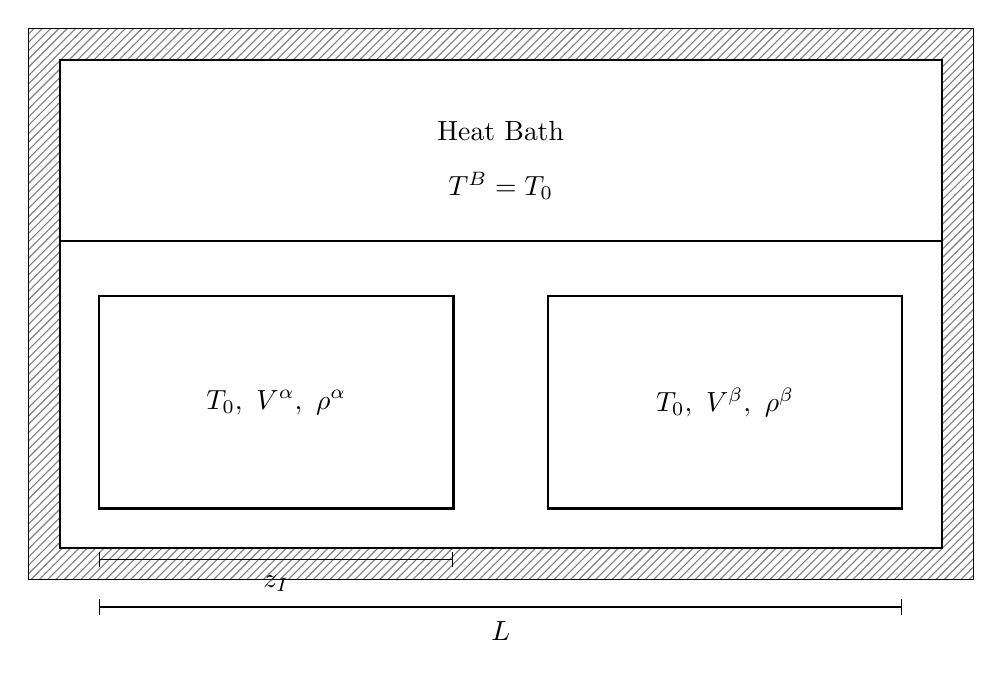
\begin{tikzpicture}
    % Outer insulated boundary
    \draw[pattern=north east lines, pattern color=black!50] (0,0) rectangle (12,7);
    \fill[white] (0.4,0.4) rectangle (11.6,6.6);
    \draw[thick] (0.4,0.4) rectangle (11.6,6.6);

    % Horizontal divider (heat bath wall)
    \draw[thick] (0.4,4.3) -- (11.6,4.3);

    % Heat bath label
    \node at (6,5.7) {Heat Bath};
    \node at (6,5.0) {$T^B=T_0$};

    % Bottom phases
    \draw[thick] (0.9,0.9) rectangle (5.4,3.6);
    \draw[thick] (6.6,0.9) rectangle (11.1,3.6);

    \node at (3.15,2.25) {$T_0,\ V^\alpha,\ \rho^\alpha$};
    \node at (8.85,2.25) {$T_0,\ V^\beta,\ \rho^\beta$};

    % Length labels
    \draw[|-|] (0.9,0.25) -- (5.4,0.25);
    \node at (3.15,-0.05) {$z_I$};

    \draw[|-|] (0.9,-0.35) -- (11.1,-0.35);
    \node at (6.0,-0.65) {$L$};
\end{tikzpicture}
\end{document}
